%
%%%%%%%%%%%%%%%%%%%%%
\section{Diagrammes}
%%%%%%%%%%%%%%%%%%%%%
%
%\subsection{Cas d'utilisation}
%
\subsection{diagramme de classes}
%
Ce diagramme présente les classes de SimFoule et indique l'inclusion des fichiers.
%
\begin{center}
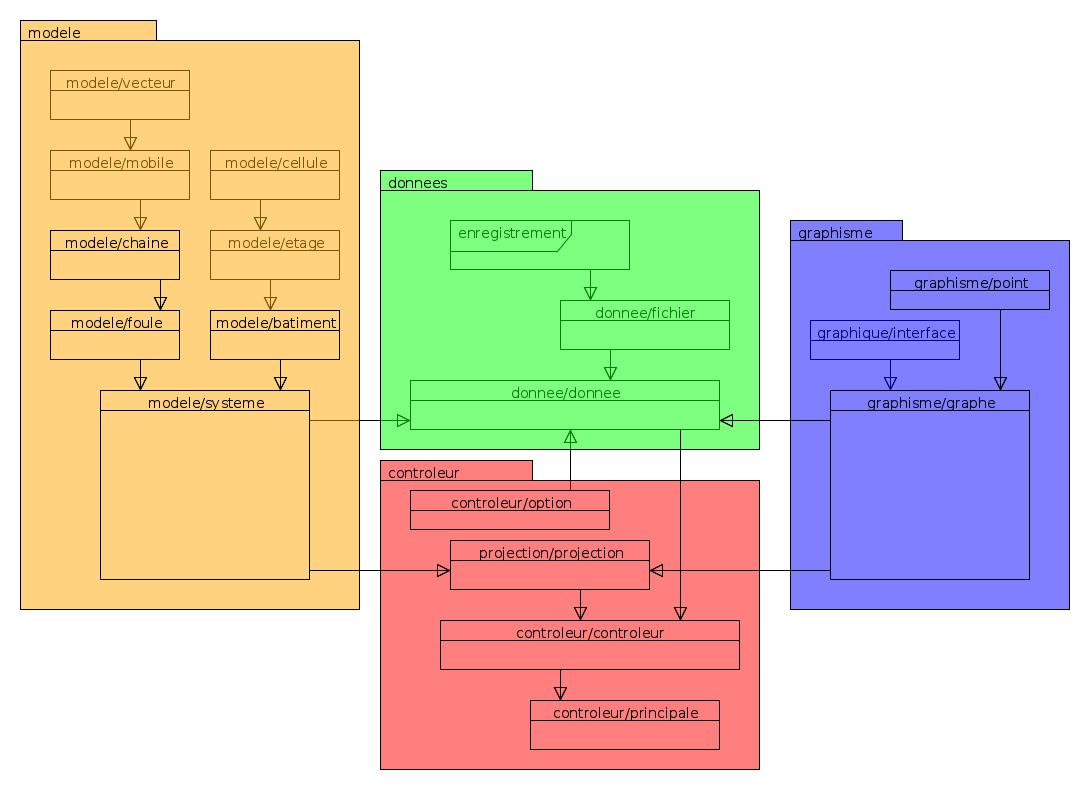
\includegraphics[scale=0.45]{./illustration/classesSimFoule}
\end{center}
%
%
\subsection{diagrammes de séquences}
%
\subsubsection{Simulation graphique}
\begin{center}
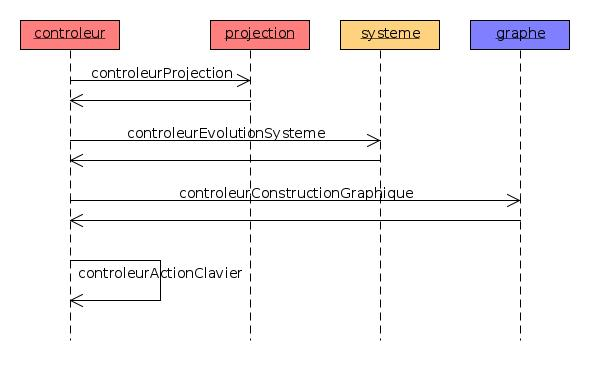
\includegraphics[scale=0.51]{./illustration/sequenceControleur}
\end{center}
%
\subsubsection{Réinitialisation}
\begin{center}
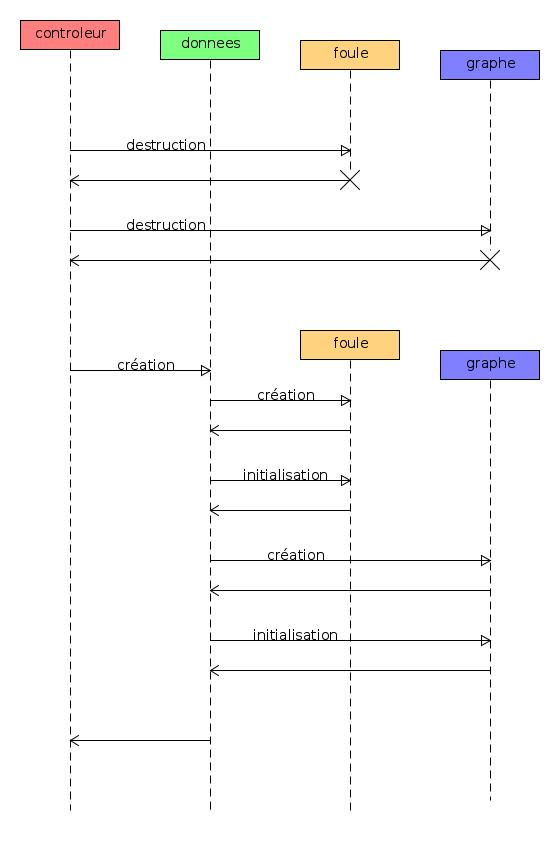
\includegraphics[scale=0.51]{./illustration/sequenceReinitialisation}
\end{center}
%
%%%%%%%%%%%%%%%%%%%%%%%%%%%%%%%%%%%%%%%%%%%%
%%%%%%%%%%%%%%%%%%%%%%%%%%%%%%%%%%%%%%%%%%%%
%\begin{itemize}[leftmargin=2cm]
%\item \texttt{gras} : texte
%\end{itemize}



%%%%%%%%%%%%%%%%%%%%%%%%%%%%%%%%%%%%%%%%%%%%%%%%%%%%%%%%%%%%%%%%%%%%%%%%%%%%%%%%%%%%%
